\documentclass[10pt]{Beamer}
\usepackage{fancybox}
\usepackage[most]{tcolorbox}
\usepackage{tikz}
\usepackage[utf8]{inputenc}
\usepackage{graphicx}



\usetheme{Frankfurt}
\usecolortheme{seahorse}
\usefonttheme{serif}


\title [Apresentação]{Apresentação: Planos de Saúde e a Teoria da Informação Assimétrica}

\author{Lorenzo Costa Miranda \& Tarcisio Iago}

\institute{UFT Palmas}

\date{\today}

\begin{document}

\frame{\titlepage}
\frame{\tableofcontents}

\section{Objetivo do Artigo}
\frame{
\frametitle{Objetivo do Artigo}

\begin{itemize}

\begin{block}
	
\item Discutir o mercado de planos e seguro-saúde utilizando a teoria da informação.

\end{block}


\begin{block}
	
\item Evidenciar o mercado de \textit{health care} no Brasil, o sistema de saúde pública e a criação da agência nacional de saúde suplementar. 

\end{block}
\end{itemize}
}


\section{Métodos}
\frame{
\frametitle{Métodos}

\begin{itemize}

\begin{block}

\item O artigo expõe a evolução do mercado de seguros de saúde ao longo do tempo, evidencia os problemas de informação intrínsecos a ele e com base nisso, analisa como procede no caso brasileiro e todas as tentativas de contornar essa barreira. 

\end{block}

\end{itemize}


}

\section{Introdução}
\frame{
\frametitle{Introdução}
	
\begin{itemize}
		
\item Origem do mercado de seguros. 
		
\vskip0,5cm	
		
\item Demanda por serviços de saúde.
		
\vskip0,5cm
		
\item O setor de saúde tem algumas peculiaridades.
		
\vskip0,5cm
		
\item Como funciona esse mercado.	
		
\end{itemize}

\begin{figure}[b]
	\centering
	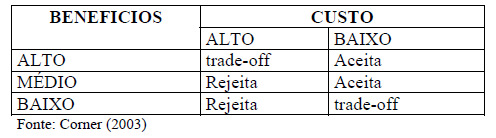
\includegraphics[width=0.6\textwidth]{tradeoff}
\end{figure}

}

\frame{
\frametitle{Introdução} 

\begin{figure}[h]
	\centering
	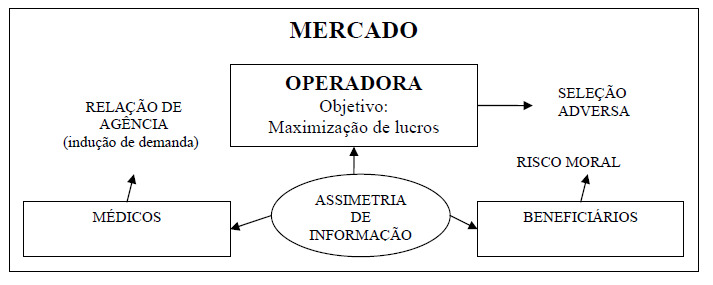
\includegraphics[width=1.0\textwidth]{problemas}
\end{figure}

}

\section{Contribuição do Artigo}
\frame{
\frametitle{A Teoria da Informação (OBJV-1)}

\shadowbox{Características Inerentes ao Mercado de Saúde}

\begin{itemize}
	
\vskip0,5cm	
	
\item[(i)] \underline{Demanda de serviços de saúde.}

\vskip0,5cm	

\item[(ii)] \underline{Comportamento esperado dos médicos.}

\vskip0,5cm	

\item[(iii)] \underline{Incerteza do produto.}

\vskip0,5cm	

\item[(iv)] \underline{Condições de oferta.}

\vskip0,5cm	

\item[(v)] \underline{Prática de preços}

\end{itemize}

}



\frame{
\frametitle{A Teoria da Informação (OBJV-1)}

\shadowbox{Risco Moral}

\begin{itemize}
	
\item Ex-ante

\vskip0,5cm	

\item Ex-post

\vskip0,5cm	

\item Co-pagamento

\vskip0,5cm	

\item Managed Care	
	
\end{itemize}	

}

\frame{
\frametitle{A Teoria da Informação (OBJV-1)}

\begin{figure}[h]
	\centering
	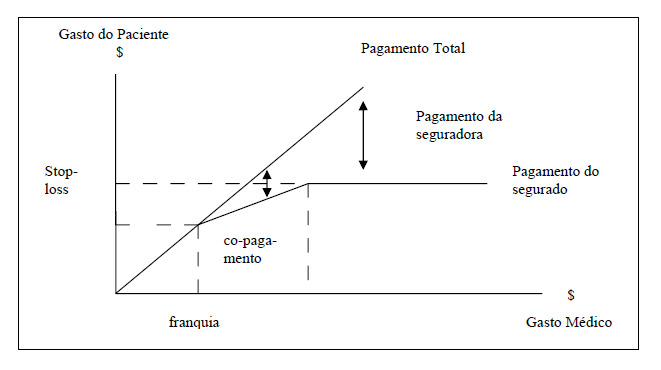
\includegraphics[width=1.0\textwidth]{copagamento}
\end{figure}



}

\frame{
\frametitle{A teoria da Informação (OBJV-1)}

\shadowbox{Seleção Adversa}

\vskip0,5cm	

\begin{itemize}

\item Os Questionários não são uma opção.

\vskip0,5cm	

\item O que se deve fazer.

\vskip0,5cm	

\item O que auxilia nos desafios de desinformação.

\vskip0,5cm	

\item A relação Agente-Principal.

\end{itemize}

}

\frame{
\frametitle{O mercado de \textit{Helth Care} no Brasil (OBJV-2)}



\shadowbox{Sistema de Saúde Brasileiro}

\begin{itemize}

\begin{block}

\item[(1)] Sistema Público - SUS.

\end{block}

\begin{block}

\item[(2)] O Setor de Saúde Suplementar.

\end{block}

\end{itemize}

}

\frame{
\frametitle{O mercado de \textit{Helth Care} no Brasil (OBJV-2)}

\shadowbox{População Assistida}

}

\frame{
\frametitle{O mercado de \textit{Helth Care} no Brasil (OBJV-2)}

\shadowbox{As Modalidades de Contrato}

\shadowbox{Considerações Finais}

}

\end{document}